% После прочтения аналит. части человек должен сделать вывод о применимости конкретного алгоритма в его конкретной ситуации

% В аналитической части описать условия применимости алгоритма в принципе (примеры и контрпримеры - при наличии доступного объема текста)

% Таблица в конце аналитического раздела

% Констр. + аналит.: на вход - информация о полигонах

\newpage
\section{Аналитический раздел}

\subsection{Представление объектов}

Существует множество способов представления трехмерных объектов в пространстве.
Наиболее популярные из них: каркасное, поверхностное и твердотельное.

\textbf{Каркасная модель} -- объекты представляются в виде набора вершин и
ребер (точек и линий). Самый простой способ и наименее требовательный к памяти
из всех рассматриваемых.

\textbf{Поверхностная модель} -- объекты представляются в виде набора
поверхностей. Поверхность, в свою очередь, также можно задать несколькими
способами, например, уравнением или набором плоскостей, аппроксимирующим
исходную поверхность. Сложные объекты часто бывает сложно или даже невозможно
описать в виде системы уравнений, а аппроксимировать, с другой стороны,
возможно всегда. \cite{m3m}

\textbf{Твердотельная модель} -- существует два самых популярных метода
представления твердотельных моделей:
\begin{enumerate}
    \item Метод конструктивного представления (англ. Constructive representation, сокращённо C-rep);
    \item Метод граничного представления (англ. Boundary representation, сокращённо B-rep).
\end{enumerate}
Первый метод заключается в комбинировании базовых составляющих элементов,
называемых твердотельными примитивами и осуществления между ними операций
пересечения, объединения и разности для построения твердотельных моделей.
Второй метод позволяет создавать точное представления твердого тела. Он хранит
точное описание границ модели, всех поверхностей и вершин. Твердотельные модели
наиболее требовательны к памяти, но позволяют точно описывать объекты, из-за
чего повсеместно используются в инженерной промышленности. \cite{msbm}

В разрабатываемой программе обнаружения коллизий нет надобности в точном
описании объектов, и каркасной модели будет достаточно.

\subsection{Формализация объектов синтезируемой сцены}

\begin{itemize}
    \item \textbf{Точечный источник света} -- точка в пространстве, излучающая свет во всех направлениях. Интенсивность света убывает по мере удаления от источника. Точечный источник света характеризуется:
        \begin{enumerate}[label=(\alph*)]
            \item Положением в пространстве (трехмерные координаты)
            \item Цветом ({RGB})
            \item Интенсивностью \textbf{I} (действительное число от $0$ до $1$)
            % \item Начальной интенсивностью \textbf{I} (действительное число от $0$ до $1$)
            % \item Функцией спада интенсивности в зависимости от расстояния до источника света (постоянная, линейная, квадратичная)
            % \item Радиусом действия \textbf{R} (на границе радиуса действия функция спада интенсивности обращается в нуль)
            \item Направлением (когда источник света расположен в бесконечности)
        \end{enumerate}
        % Функции спада интенсивности имеют вид:
        % \begin{itemize}
        %     \item Постоянная: $ f(x) = {I},\ 0 \leq x \leq {R} $
        %     \item Линейная: $ f(x) = {I} \cdot \left( 1 - \frac{x}{{R}} \right),\ 0 \leq x \leq {R} $
        %     \item Квадратичная: $ f(x) = {I} \cdot \left( 1 - \frac{x}{{R}} \right)^2,\ 0 \leq x \leq {R} $
        % \end{itemize}
    \item \textbf{Объект сцены} -- набор трехмерных примитивов, формирующих полигональную сетку. Объект сцены характеризуется:
        \begin{enumerate}[label=(\alph*)]
            \item Положением в пространстве (трехмерные координаты)
            \item Ориентацией в пространстве (матрица модели)
            \item Цветом ({RGB})
        \end{enumerate}
    \item \textbf{Земля} -- {объект сцены}, представляющий собой рельефную территорию.
    \item \textbf{Плоскость Земли} -- горизонтальная плоскость (параллельная {XY}), проходящая через самую низкую точку {Земли}.
    \item \textbf{Камера} характеризуется:
        \begin{enumerate}[label=(\alph*)]
            \item Положением в пространстве (трехмерные координаты)
            \item Направлением взгляда (трехмерный вектор)
            \item Ориентацией в пространстве (трехмерный вектор, указывающий, в каком направлении у камеры верх)
            \item Расстояниями до ближней и дальней граней пирамиды видимости
            \item Углом обзора
            \item Соотношением сторон
        \end{enumerate}
\end{itemize}

\subsection{Анализ алгоритмов удаления невидимых линий и поверхностей}

Алгоритмы удаления невидимых линий и поверхностей можно разделить на две
группы. Одни работают в объектном пространстве -- для каждого объекта
проверяется, заслоняют ли его другие объекты или нет. Таким образом,
потребуется $O(n^2)$ сравнений объектов. К таким алгоритмам относится,
например, алгоритм Робертса. Другие работают в пространстве изображения -- для
каждого пикселя изображения определяется, какой объект сцены в нём виден. То
есть, потребуется $O(Nn)$ сравнений, где $N$ -- количество пикселей. Таковы
алгоритмы трассировки лучей, Варнока или $z$-буфера.

На первый взгляд может показаться, что, если мы редко имеем дело с более чем
$1920 \times 1080$ объектами, то эффективнее будет использовать алгоритм,
работающий в объектном пространстве, чтобы было меньше сравнений, однако это
далеко не всегда так.

\subsubsection{Алгоритм Робертса}

Одно из требований алгоритма -- тела должны быть выпуклыми. Поэтому, если
какие-то из объектов сцены не выпуклые, то их следует разбить на выпуклые
составляющие. На последующих этапах алгоритма удаляются:
\begin{enumerate}
    \item Невидимые рёбра, экранируемые самим телом;
    \item Невидимые рёбра, экранируемые другими телами сцены;
    \item Новые невидимые рёбра, возникающие при <<протыкании>> тел друг
        другом.
\end{enumerate}

К преимуществам данного алгоритма можно отнести его математическую точность и
простоту идеи. \cite[с.~250]{rogers}

К недостаткам -- следующие:\begin{enumerate}
    \item Трудности при работе с невыпуклыми объектами; их нужно разделять на
        выпуклые составляющие, что само по себе задача трудоёмкая.
    \item Для каждого выпуклого тела составляется матрица размерности $4 \times
        N$, где $N$ -- количество граней тела. Если в программе используются
        модели с большим количеством полигонов, эта матрица может быть очень
        большой, и выполнение операций над ней может значительно повлиять на
        время генерации кадра.
    \item После разбиения объектов на выпуклые составляющие, количество
        объектов, для которых нужно выполнить проверку перекрытия возрастает,
        что увеличивает время выполнения алгоритма.
\end{enumerate}

\subsubsection{Алгоритм обратной трассировки лучей}

Суть алгоритма для обработки скрытых или видимых поверхностей следующая:
выпускаем луч через каждый пиксель перпендикулярно плоскости экрана и следим за
его траекторией до тех пор, пока он не пересечёт поверхность видимого
непрозрачного тела. Необходимо проверить пересечение каждого объекта сцены с
каждым лучом, далее пересечения упорядочиваются по глубине. Пересечение с
максимыльным значением $z$ представляет видимую поверхность для данного
пикселя. \cite[с.~362]{rogers}

Процедура поиска пересечений играет ключевую роль в алгоритме трассировки
лучей, поскольку $75-95\%$ времени выполнения алгоритма приходится на неё. В
связи с этим существуют многие оптимизации алгоритма, позволяющие не искать
пересечения для объектов, которые луч точно не пересечёт. Например, заключение
объекта или кластера объектов в сферическую или прямоугольную оболочки и
проверка пересечения с оболочкой; если пересечения с оболочкой нет, значит луч
не пересекает и объекты, в ней содержащиеся. \cite[с.~363]{rogers}

Преимуществом данного алгоритма является его независимость от характеристик
когерентности той сцены, для которой ведётся поиск её видимых участков.
Рассчёты для каждого пикселя производятся отдельно, независимо от других,
следовательно, имеется возможность выполнять вычисления параллельно.

Ещё одним преимуществом алгоритма является возможность учёта прозрачности
объектов при некоторой его модификации.

\subsubsection{Алгоритм Варнока}

Алгоритм основывается на рекурсивном разбиении экрана и работает тем быстрее,
чем меньше на экране пересечений объектов. Подробнее преимущества и недостатки
алгоритма будут рассмотрены в таблице.

\subsubsection{Алгоритм, использующий $z$-буфер}

Алгоритм работает следующим образом:
\begin{enumerate}
    \item Создаётся $z$-буфер, размерность которого равна размерности буфера
        кадра, и инициализируется минимальными значениями $z$.
    \item В процессе работы глубина или значение z каждого нового пиксела,
        который нужно занести в буфер кадра, сравнивается с глубиной того
        пиксела, который уже занесен в $z$-буфер. Если это сравнение
        показывает, что новый пиксел расположен впереди пиксела, находящегося в
        буфере кадра, то новый пиксеп заносится в этот буфер и производится
        корректировка $z$-буфера новым значением $z$. \cite[с.~321]{rogers}
\end{enumerate}

Данный алгоритм может эффективно обрабатывать сложные сцены, но при этом
требует большой объём памяти для хранения $z$-буфера и немалые вычислительные
мощности -- при его обновлении. Также, в связи с произвольным порядком
сравнения объектов, возникают сложности с учётом их прозрачности.

\subsubsection{Вывод}

\noindent
\begin{adjustbox}{width=1\textwidth}
    \begin{tabular}{|p{.25\textwidth}|p{.25\textwidth}|p{.25\textwidth}|p{.25\textwidth}|p{.25\textwidth}|}
        \hline
        &
        Алгоритм Робертса
        &
        Алгоритм обратной трассировки лучей
        &
        Алгоритм Варнока
        &
        Алгоритм, использующий $z$-буфер
        \\
        \hline
        Рабочее пространство
        &
        % Алгоритм Робертса
        Объектное
        &
        % Алгоритм обратной трассировки лучей
        Изображения
        &
        % Алгоритм Варнока
        Изображения
        &
        % Алгоритм, использующий Z-буфер
        Изображения
        \\
        \hline
        Асимптотическая сложность алгоритма ($n$ -- количество граней объектов,
        $N$ -- количество пикселей)
        &
        % Алгоритм Робертса
        \cellcolor{black!12}
        $O(n^2)$
        &
        % Алгоритм обратной трассировки лучей
        \cellcolor{black!12}
        $O(Nn)$
        &
        % Алгоритм Варнока
        \cellcolor{black!12}
        $O(Nn)$
        &
        % Алгоритм, использующий Z-буфер
        \cellcolor{black!12}
        $O(Nn)$
        \\
        \hline
        Возможность выполнять вычисления параллельно для каждого пикселя
        &
        % Алгоритм Робертса
        \cellcolor{black!25}
        Нет
        &
        % Алгоритм обратной трассировки лучей
        \cellcolor{black!5}
        Есть
        &
        % Алгоритм Варнока
        \cellcolor{black!25}
        Нет
        &
        % Алгоритм, использующий Z-буфер
        \cellcolor{black!5}
        Есть
        \\
        \hline
        Возможность учёта прозрачности объектов
        &
        % Алгоритм Робертса
        \cellcolor{black!25}
        Нет
        &
        % Алгоритм обратной трассировки лучей
        \cellcolor{black!5}
        Есть 
        &
        % Алгоритм Варнока
        \cellcolor{black!25}
        Нет
        &
        % Алгоритм, использующий Z-буфер
        \cellcolor{black!12}
        Есть (но сложно наладить корректную работу)
        \\
        \hline
        Эффективность не зависит от сложности сцены
        &
        % Алгоритм Робертса
        \cellcolor{black!25}
        Нет
        &
        % Алгоритм обратной трассировки лучей
        \cellcolor{black!5}
        Да
        &
        % Алгоритм Варнока
        \cellcolor{black!25}
        Нет
        &
        % Алгоритм, использующий Z-буфер
        \cellcolor{black!5}
        Да
        \\
        \hline
        Эффективность обработки сложных сцен
        &
        % Алгоритм Робертса
        \cellcolor{black!25}
        Низкая
        &
        % Алгоритм обратной трассировки лучей
        \cellcolor{black!12}
        Средняя
        &
        % Алгоритм Варнока
        \cellcolor{black!25}
        Низкая
        &
        % Алгоритм, использующий Z-буфер
        \cellcolor{black!5}
        Высокая
        \\
        \hline
        Сложность реализации
        &
        % Алгоритм Робертса
        \cellcolor{black!5}
        Низкая
        &
        % Алгоритм обратной трассировки лучей
        \cellcolor{black!12}
        Средняя
        &
        % Алгоритм Варнока
        \cellcolor{black!12}
        Средняя
        &
        % Алгоритм, использующий Z-буфер
        \cellcolor{black!5}
        Низкая
        \\
        \hline
    \end{tabular}
\end{adjustbox}

\vspace{0.5cm}

В программе обнаружения коллизий важную роль имеет скорость генерации кадра и
менее важную -- реалистичность изображения, которую можно было бы повысить,
используя алгоритм обратной трассировки лучей. В связи с этим фактом и
результатами, отображёнными в таблице выше, для удаления невидимых линий и
поверхностей в программе был выбран алгоритм, использующий $z$-буфер.

\subsection{Анализ алгоритмов обнаружения коллизий}

\subsubsection{Алгоритм AABB}

Алгоритм ограничивающего параллепипеда с гранями, выравненными по осям
координат (англ. Axis-Aligned Bounding Box algorithm, сокращённо AABB)
заключается в ограничении объектов параллелепипедами с гранями, выравненными по
осям координат и последующем обранужении коллизий, используя теорему о
разделяющей гиперплоскости \cite{hpst}. То, что грани обоих AABB гарантированно
параллельны общему набору осей координат, говорит о том, что разделяющая ось,
если таковая существует, будет одной из этих осей координат \cite[с.~827]{gea}.
Обнаружение пересечений двух AABB-параллелепипедов очень просто в связи с
параллельностью их граней координатным плоскостям: если проекции
параллелепипедов на каждую координатную плоскость пересекаются, то пересекаются
и сами параллелепипеды, иначе -- пересечения нет.

\subsubsection{Алгоритм OBB}

В алгоритме ориентированного ограничивающего параллелепипеда (англ. Oriented
Bounding Box algorithm, сокращённо OBB), в отличие от AABB, объекты
ограничиваются параллелепипедом, грани которого не обязательно параллельны
координатным плоскостям. Обнаружение пересечений двух OBB-параллелепипедов
сложнее, чем для AABB-параллелепипедов, но в его основе также лежит теорема о
разделяющей гиперплоскости \cite{hpst}, суть которой заключается в том, что
проекции двух фигур на разделяющую плоскость не пересекаются, если не
пересекаются сами фигуры. Проекции этих же фигур на неразделяющую ось могут
пересекаться.

\begin{figure}[h]
    \caption{Обнаружение пересечений двух OBB-прямоугольников. \cite[102]{rtcd}}
    \noindent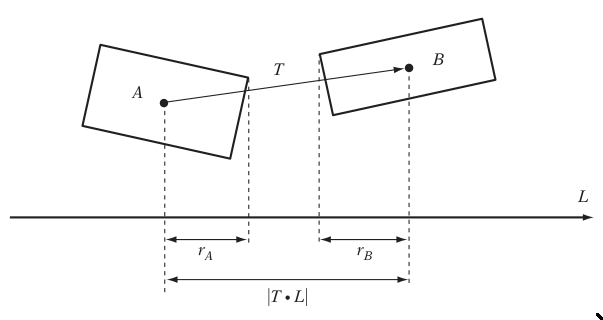
\includegraphics[width=\linewidth]{img/OBB-test.jpg}
    \label{fig:obb-test}
\end{figure}

Тест на обнаружение пересечений двух OBB-параллелепипедов следующий: Два
OBB-параллелепипеда не пересекаются, если сумма проекций их радиусов на
разделяющую ось меньше расстояния между проекциями их центров
(Рис.~\ref{fig:obb-test}).

\subsubsection{Алгоритм GJK}

Алгоритм Гильберта -- Джонсона -- Кирти (англ. Gilbert -- Johnson -- Keerthi
algorithm, сокращённо GJK) основан на геометрической операции, известной как
\textit{Разность Минковского}. Она довольно проста: мы берём каждую точку
внутри формы $B$ и последовательно вычитаем её из каждой точки внутти формы
$A$. Полученное множество точек $\left\{\left( \mathbf{A}_i - \mathbf{B}_j
\right)\right\}$ и будет разностью Минковского. \cite[с.~829]{gea}

У разности Минковского есть одно полезное свойство: если применить её к двум
выпуклым формам, она будет \textit{содержать начало координат} тогда и только
тогда, когда эти две формы пересекаются. Можно интуитивно понять, почему оно
является верным: под пересечением форм $A$ и $B$ на самом деле имеется в виду,
что внутри $A$ есть такие точки, которые находятся также внутри $B$. Вычитая
каждую точку, составляющую $B$, из каждой точки, составляющей $A$, мы можем
ожидать, что в какой-то момент нам попадется точка, общая для двух форм. В
таком случае вычитание даст ноль, поэтому разность Минковского будет содержать
начало координат тогда и только тогда, когда формы $A$ и $B$ имеют общие точки.

Разность Минковского для двух выпуклых форм сама является выпуклой формой. Но
нас интересует лишь её оболочка, а не все её внутренние точки. Основной принцип
работы $GJK$ состоит в поиске тетраэдра, размещённого на оболочке разности
Минковского и включающего в себя начало координат. Если такую фигуру можно
найти, формы пересекаются, в противном случае -- нет. \cite[с.~830]{gea}

Подробнее с алгоритмом помогут ознакомиться следующие источники: \cite{gjksm},
\cite{gjkppt1}, \cite{gjkppt2}, \cite{gjk}.

\subsubsection{Вывод}

\noindent
\begin{adjustbox}{width=1\textwidth}
    \begin{tabular}{|p{.25\textwidth}|p{.25\textwidth}|p{.25\textwidth}|p{.25\textwidth}|p{.25\textwidth}|}
        \hline
        &
        Алгоритм GJK
        &
        Алгоритм AABB
        &
        Алгоритм OBB
        \\
        \hline
        Асимптотическая сложность ($n$ -- количество вершин в полигональном
        представлении объекта)
        &
        % Алгоритм GJK
        \cellcolor{black!12}
        $O(n^2)$ (худшее)
        &
        % Алгоритм AABB
        \cellcolor{black!5}
        $O(1)$
        &
        % Алгоритм OBB
        \cellcolor{black!12}
        $O(n^2)$ (худшее)
        \\
        \hline
        Точность обнаружения коллизий
        &
        % Алгоритм GJK
        \cellcolor{black!5}
        Высокая
        &
        % Алгоритм AABB
        \cellcolor{black!25}
        Низкая
        &
        % Алгоритм OBB
        \cellcolor{black!12}
        Средняя
        \\
        \hline
        Эффективность на сложных формах
        &
        % Алгоритм GJK
        \cellcolor{black!5}
        Высокая
        &
        % Алгоритм AABB
        \cellcolor{black!25}
        Низкая
        &
        % Алгоритм OBB
        \cellcolor{black!12}
        Средняя
        \\
        \hline
        Сложность реализации
        &
        % Алгоритм GJK
        \cellcolor{black!25}
        Высокая
        &
        % Алгоритм AABB
        \cellcolor{black!5}
        Низкая
        &
        % Алгоритм OBB
        \cellcolor{black!12}
        Средняя
        \\
        \hline
    \end{tabular}
\end{adjustbox}

\vspace{0.5cm}

В программе для обнаружения коллизий важнейшими критериями при выборе алгоритма
являются точность обнаружения коллизий и его эффективность на сложных формах. В
связи с этим был выбран алгоритм $GJK$, несмотря на сложность его реализации.
